\documentclass[12pt,a4paper]{article}
\usepackage[polish]{babel}
\usepackage[T1]{fontenc}
\usepackage[utf8x]{inputenc}
\usepackage{hyperref}
\usepackage{url}
\usepackage[]{algorithm2e}
\usepackage{listings}
\usepackage{tcolorbox}

\usepackage{color}
\usepackage{listings}

\lstloadlanguages{% Check Dokumentation for further languages ...
	C,
	C++,
	csh,
	Java,
	Python
}
\usepackage{tikz}
\usetikzlibrary{mindmap}

\definecolor{red}{rgb}{0.6,0,0} % for strings
\definecolor{blue}{rgb}{0,0,0.6}
\definecolor{green}{rgb}{0,0.8,0}
\definecolor{cyan}{rgb}{0.0,0.6,0.6}

\newenvironment{blockquote}{%
  \par%
  \medskip
  \leftskip=4em\rightskip=2em%
  \noindent\ignorespaces}{%
  \par\medskip}

\lstset{
	language=bash,
	basicstyle=\footnotesize\ttfamily,
	numbers=left,
	numberstyle=\tiny,
	numbersep=5pt,
	tabsize=2,
	extendedchars=true,
	breaklines=true,
	frame=b,
	stringstyle=\color{blue}\ttfamily,
	showspaces=false,
	showtabs=false,
	xleftmargin=17pt,
	framexleftmargin=17pt,
	framexrightmargin=5pt,
	framexbottommargin=4pt,
	commentstyle=\color{green},
	morecomment=[l]{//}, %use comment-line-style!
	morecomment=[s]{/*}{*/}, %for multiline comments
	showstringspaces=false,
	morekeywords={ abstract, event, new, struct,
		as, explicit, null, switch,
		base, extern, object, this,
		bool, false, operator, throw,
		break, finally, out, true,
		byte, fixed, override, try,
		case, float, params, typeof,
		catch, for, private, uint,
		char, foreach, protected, ulong,
		checked, goto, public, unchecked,
		class, if, readonly, unsafe,
		const, implicit, ref, ushort,
		continue, in, return, using,
		decimal, int, sbyte, virtual,
		default, interface, sealed, volatile,
		delegate, internal, short, void,
		do, is, sizeof, while,
		double, lock, stackalloc,
		else, long, static,
		enum, namespace, string},
	keywordstyle=\color{cyan},
	identifierstyle=\color{red},
}
\usepackage{caption}
\DeclareCaptionFont{white}{\color{white}}
\DeclareCaptionFormat{listing}{\colorbox{blue}{\parbox{\textwidth}{\hspace{15pt}#1#2#3}}}
\captionsetup[lstlisting]{format=listing,labelfont=white,textfont=white, singlelinecheck=false, margin=0pt, font={bf,footnotesize}}


\addtolength{\hoffset}{-1.5cm}
\addtolength{\marginparwidth}{-1.5cm}
\addtolength{\textwidth}{3cm}
\addtolength{\voffset}{-1cm}
\addtolength{\textheight}{2.5cm}
\setlength{\topmargin}{0cm}
\setlength{\headheight}{0cm}

\begin{document}
	
	\title{Języki Skryptowe\\\small{dokumentacja projektu Zegar 2010}}
	\author{Marceli Pychyński, grupa 3F, Wydział Matematyki Stosowanej - Informatyka semeste 3}
	\date{\today}

	\maketitle
	\newpage
	
	\tableofcontents
	
	\newpage
	\section{Opis problemu przedstawionego w zadaniu}
	
    	\subsection{Treść zadania}
        	W zadaniu rozważamy zegar, który wskazuje na godzinę 12:00. Należy obliczyć ile minie sekund, do ponownego ustawienia się wskazówek w jednej linii. Największym problem jest to, że wskazówki pokonują drogę po okręgu w różnym czasie, a wskazówka minutowa „goni”/podąża za wskazówką godzinową. Dalsza część opisu problemu zawarta jest w modelu matematyczny, ponieważ w trakcie rozważań wyprowadzany jest wzór potrzebny do rozwiązania zadania.
        
        
        \subsection{Założenia}
        
            Wejście - \textbf{plik: input.txt}
            \begin{blockquote}
                Pierwsza linią tego pliku jest licznik wyznaczonego w modelu matematycznym pierwiastka.Drugą linią tego pliku jest mianownik ww. pierwiastka.
            \end{blockquote}
            
            \noindent Wyjście 1 - \textbf{plik: output.txt}
            
            \begin{blockquote}
                Pierwsza linią tego pliku jest obliczony czas w sekundach, a drugą linią tego pliku jest przeliczony czas z sekund na format godzina, minuta, sekunda milisekunda.
                \end{blockquote}
                
            \noindent Wyjście 2 - \textbf{plik: output.html}
                \begin{blockquote}
                Plik zawiera czytelną tabelę stworzoną w html'u z zawartymi wynikami z output.txt
                \end{blockquote}
                
            
            
        
        \subsection{Przykładowy format danych wejściowych i wyjściowych}
        
            \textbf{input.txt}
            \begin{blockquote}
                12\\
                11
            \end{blockquote}
                
            \noindent\textbf{output.txt}
            \begin{blockquote}
                3927.272727272727\\
                1 h 5 m 27 s 27 ms
            \end{blockquote}
            
            \noindent\textbf{output.html}
            \begin{blockquote}
                Tabela z danymi wejściowym i wyjściowymi
            \end{blockquote}
    
    
    \section{Model Matematyczny}
        \subsection{Problem}
            \begin{tcolorbox}
                W ciągu 12h wskazówka godzinowa pokonuje cały okrąg, zatem w 1h pokona  1/12 okręgu, ponieważ na wskazówce minutowej, przejście całego okręgu zajmuje 12h. Z tego wynikają dane (m – minutowa, g – godzinowa): $t_{m}=1h$, $t_{g}=12h$
            \end{tcolorbox}
            
            \begin{figure}
                \hfill
                \subfigure{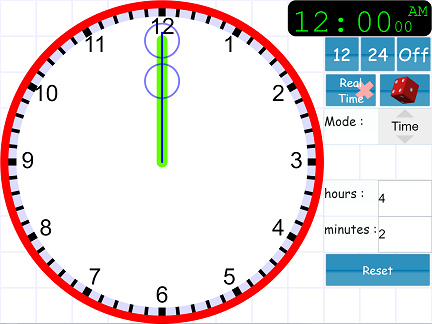
\includegraphics[width=6cm]{Zegar1.PNG}}
                \hfill
                \subfigure{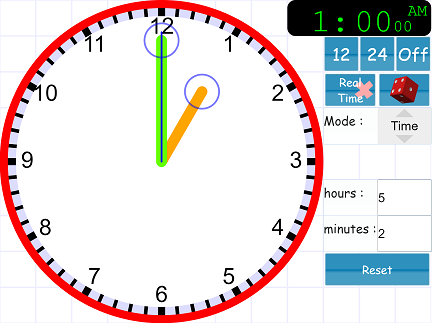
\includegraphics[width=6cm]{Zegar2.PNG}}
                \hfill
                \caption{Porównanie zegarów w godzinach 12:00 i 13:00}
            \end{figure}
            
                        \begin{figure}
                \hfill
                \subfigure{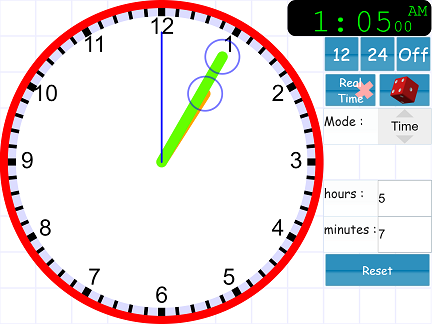
\includegraphics[width=6cm]{Zegar3.PNG}}
                \hfill
                \subfigure{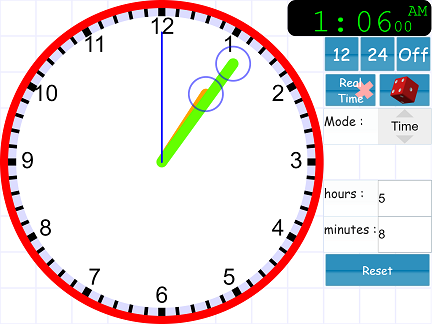
\includegraphics[width=6cm]{Zegar4.PNG}}
                \hfill
                \caption{Porównanie zegarów w godzinach 13:05 i 13:06}
            \end{figure}
            
            \begin{blockquote}
                W takim razie, po 1h będzie 13:00. Wskazówki będą od siebie w „odległości” 5 minut (godzinowa na: 1, minutowa na: 0), więc po 5 minutach wskazówka minutowa zbliży się bardzo blisko do wskazówki godzinowej, ale nie najdą na siebie,ponieważ w ciągu tych 5 minut wskazówka godzinowa pokona 2.5 stopnia (wynika to z prędkości kątowej (360°)/12h ).
             \end{blockquote}
             
             \begin{blockquote}
                \begin{center}
                  $  s_{m} \neq s_{g}$ \\
                \end{center}
                  Aby wyprowadzić wzór na miejsce spotkania, można do drogi wskazówki godzinowej dodać 2π, ponieważ pokonała drogę krótsza o przynajmniej jeden okrąg.
                 \begin{center}
                  $  s_{m} = s_{g} + 2\pi$ \\
                \end{center}
            \end{blockquote}
            
            \begin{blockquote}
                Jednak bez obliczenia, nie jesteśmy w stanie określić dokładnie, na której sekundzie wskazówki ustawią się w jednej linii.
            \end{blockquote}
            
            \begin{blockquote}
                Po krótkiej analizie można uznać, że najlepszą drogą jest tak naprawdę zakreślony kąt (czyli $s_{m}=\alpha_{m}$
                i $s_{g}=α_{g}$, a takie dane z jakimi się spotkaliśmy można wykorzystać do zastosowania wzoru na prędkość kątową
            \end{blockquote}
            
            \begin{blockquote}
                Ze wzoru na prędkość kątową  $\omega= \frac{\alpha}{t} $, można wyprowadzić wzór $\alpha = \omega*t$ \\\\
                $\omega$ – prędkość kątowa \\
                $\alpha$ – zakreślony kąt \\
                t – czas pokonania
            \end{blockquote}
            
            \begin{blockquote}
                Teraz zamieniamy $s_{m} = s_{g} + 2\pi$ na:
                \begin{center}
                    $\alpha_{m} = \alpha_{g} + 2\pi$
                \end{center}
                $\alpha_{m} = \omega_{m}t$, gdzie „t” jest szukanym czasem, po którym wskazówki się pokrywają
                \begin{center}
                    $\omega_{m}t = \omega_{g}t + 2\pi$
                \end{center}
                $\omega = \frac{2\pi}{t}$, a więc:
                \begin{center}
                $\frac{2\pi}{t_{m}}t = \frac{2\pi}{t_{g}}t+2\pi$ \\
                $\frac{t}{t_{m}} = \frac{t}{t_{g}}+1$ \\
                $t(\frac{1}{t_{m}}-\frac{1}{t_{g}})=1$ \\
                $t = \frac{1}{\frac{1}{t_{m}}-\frac{1}{t_{g}}}$ \\
                \end{center}
                Teraz do wprowadznego wzoru można podstawić dane, które zostały ustalone na początku rozwiązania: \\
                \begin{center}
                $t = \frac{1}{\frac{1}{1}-\frac{1}{12}}$ \\   
                $t=\frac{12}{11} (h)$
                \end{center}
                Gdzie t jest szukanym czasem.
                
            \end{blockquote}
            
            

             

            
	\subsection{Instrukcja obsługi}
	W celu uruchomienia programów projektowy należy otworzyć plik menu.bat (uprawnienia administracyjne nie są wymagane)
	
	\begin{figure}[!htb]
	    \centering
	    
\includegraphics{menuicon.PNG}
	    \title{Ładna ikonka skrótu do pliku menu.bat}
	\end{figure}
	
	\begin{figure}[!htb]
	    \centering
	    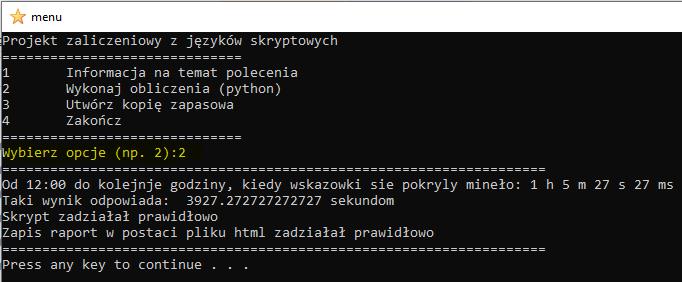
\includegraphics{menucmd.PNG}
	\end{figure}
	\newpage
	
	
	
	\subsection{Wymagania sprzętowe}
	System operacyjny Windows 10\\
	Interpreter języka Python w wersji 3.X.X
	\newpage
	\section{Algorytm}
	\subsection*{Opis działania} 
	
	Pseudokod algorytmu:
    \subsection{Pseudokod}
    \begin{algorithm}
        \KwData{Dane wejściowe: $x, y, var = res = \frac{x}{y}$}
        \KwResult{$res*60*60$}
        	Wprowadź godzinę w postaci ułamka (np. 4/3)  i zapisz do zmiennej typu rzeczywistego „var” i „res”\\
        	Do zmiennej „h” przypisz  część całkowitą zmiennej var\\
        	Do zmiennej „var” przypisz jako typ rzeczywisty wynik z działania (var-h)×60\\
        	Do zmiennej „m” przypisz część całkowitą zmiennej var\\
        	Do zmiennej „var” przypisz jako typ rzeczywisty wynik z działania (var-m)×60\\
        	Do zmiennej „s” przypisz część całkowitą zmiennej var\\
        	Do zmiennej „var” przypisz jako typ rzeczywisty wynik z działania (var-s)×100\\
        	Do zmiennej „ms” przypisz część całkowitą zmiennej var\\
        	Wypisz godzinę w postaci „h” „m” „s” „ms”\\
        	Wypisz ilość sekund używając (res*60*60)
    \end{algorithm}
	\subsection{Schemat blokowy}
	\newpage
	\begin{figure}[!htb]
	    \centering
	    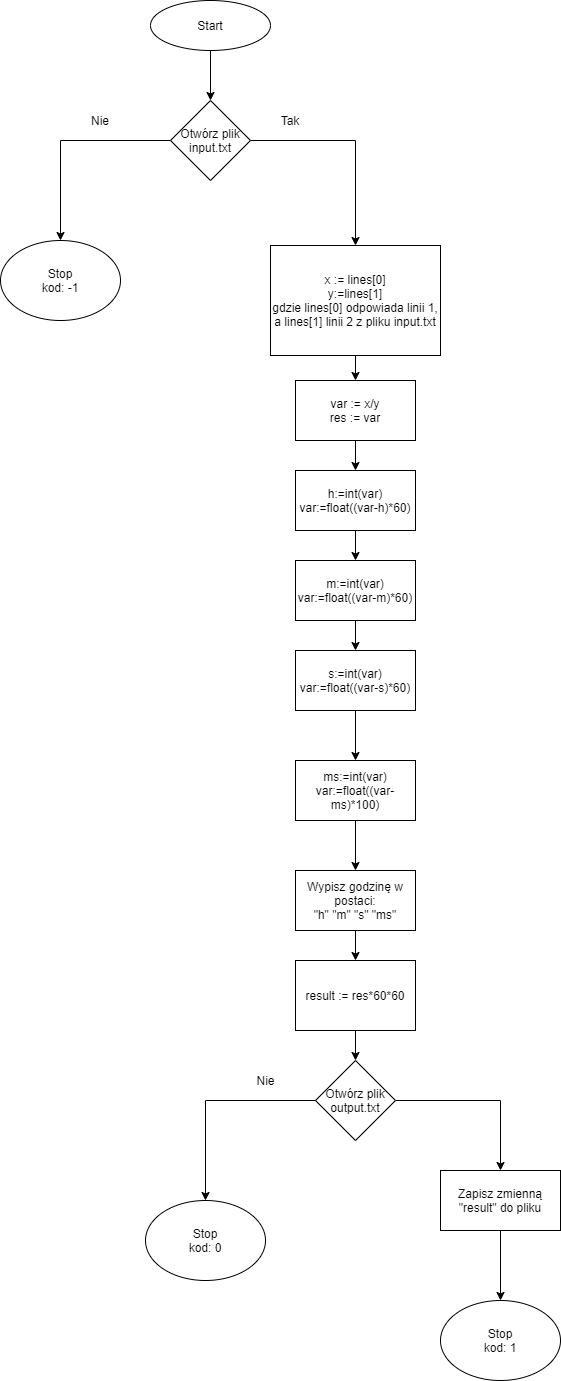
\includegraphics[scale=0.45]{Schemat.png}
	\end{figure}


	\section{Implementacja}
	Opis, zasada i działanie programu ze względu na podział na pliki, nastepnie	funkcje programu wraz ze szczegółowym opisem działania (np.: formie pseudokodu, czy odniesienia do równania) \\
	
	Program menu.bat jest skryptem systemowym, który steruję wszystkimi programami
	
	\begin{tikzpicture}[mindmap, grow cyclic, every node/.style=concept, concept color=orange!40, 
	level 1/.append style={level distance=5cm,sibling angle=90},
	level 2/.append style={level distance=3cm,sibling angle=45},]

    \node{menu.bat}
	child { node {1 Info}}
	child [concept color=green!40]{ node {3 makeHTML.py}
	    child [concept color=blue!30]{ node {Exit code: -1}}
	    child [concept color=blue!30]{ node {Exit code: 0}}
	    child [concept color=blue!30]{ node {Exit code: 1}}
	    }
	child { node {4 Exit}}
	child [concept color=green!40]{ node {2 Solve.py}
	    child [concept color=blue!30]{ node {Exit code: -1}}
	    child [concept color=blue!30]{ node {Exit code: 0}}
	    child [concept color=blue!30]{ node {Exit code: 1}}
	    }
	;
    \end{tikzpicture}
    \\Kod wyjścia 1 - skrypt zadziałał prawidłowo\\
    Kod wyjścia 0 - błąd zapisu danych\\
    Kod wyjścia -1 - błąd odczytu danych wejściowych\\\\
    
    
    \\\\menu.bat
    \begin{lstlisting}
    @echo off
    :menu
    cls
    echo Projekt zaliczeniowy z jezykow skryptowych
    echo ==============================
    echo 1	Informacja na temat polecenia
    echo 2	Wykonaj obliczenia (python)
    echo 3	Utworz kopię zapasowa
    echo 4	Zakoncz
    echo ==============================
    set /p select=Wybierz opcje (np. 2):
    IF %select%==1 GOTO opt1
    IF %select%==2 GOTO opt2
    IF %select%==3 goto opt3
    IF %select%==4 goto exit
    :opt1
    echo ====================================================================
    echo Polecenie jest nastepujace:
    echo Wskazowki zegara sa ustawione na godzine 1200 . Nalezy napisac program
    echo obliczajacy czas w sekundach jaki uplynal od momentu startu zegara do momentu
    echo ustawienia sie wskazowek w jednej linii. Wynik nalezy zapisac w pliku "output.txt".
    echo ====================================================================
    pause
    goto menu
    :opt2
    echo ====================================================================
    python solve.py
    If %ERRORLEVEL% == 1 (echo Skrypt zadzialal prawidlowo)
    If %ERRORLEVEL% == 0 (echo Blad zapisu plikow wyjsciowych)
    If %ERRORLEVEL% == -1 (echo Blad otwarcia plikow wejsciowych)
    
    python makeHTML.py
    If %ERRORLEVEL% == 1 (echo Zapis raport w postaci pliku html zadzialal prawidlowo)
    If %ERRORLEVEL% == 0 (echo Blad zapisu plikow wyjsciowych w postaci pliku html)
    If %ERRORLEVEL% == -1 (echo Blad otwarcia plikow wejsciowych podczas tworzenia raportu)
    echo ====================================================================
    
    pause
    goto menu
    :opt3
    echo ====================================================================
    echo Kopiowanie folderu %cd%...
    echo Usuwanie starej kopii zapasowej...
    rmdir /S /Q %userprofile%\Backup
    echo Tworzenie nowej kopii zapasowej...
    mkdir %userprofile%\Backup
    xcopy /e /v "%cd%" "%userprofile%\Backup"
    echo ====================================================================
    pause
    goto menu
    :exit
    echo Koniec
    pause
    \end{lstlisting}
    
    
    
    solve.py
	\begin{lstlisting}]
    	lines = []
    
    try:
        file_in = open("input.txt", "r")
        lines = file_in.readlines()
        file_in.close()
    except IOError:
        print("Nie znaleziono pliku")
        exit(-1)
    
    try:
        x = int(lines[0])
        y = int(lines[1])
    except ValueError:
        print("Nieprawidlowe dane wejsciowe, program zostanie wykonany na ponizszych danych:")
        print("licznik: 12, mianownik: 11")
        x = 12
        y = 11
    
    var = res = float(x / y)
    h = int(var)  # godziny
    var = float((var - h) * 60)
    m = int(var)  # minuty
    var = float((var - m) * 60)
    s = int(var)  # sekundy
    var = float((var - s) * 100)
    ms = int(var)
    
    result3 = "{} h {} m {} s {} ms".format(h, m, s, ms)
    result2 = ("Od 12:00 do kolejnej godziny, kiedy wskazowki sie pokryly minelo: {} h {} m {} s {} ms".format(h, m, s, ms))
    print(result2)
    result = float(res * 60 * 60)
    print("Taki wynik odpowiada: ", result, "sekundom")
    
    try:
        file_out = open("output.txt", "w")
        file_out.writelines(str(result))
        file_out.writelines("\n")
        file_out.writelines(str(result3))
        file_out.close()
    except IOError:
        print("Blad zapisu danych")
        exit(0)
    
    exit(1)

	\end{lstlisting}
	
	
	
	
	
	\\
	\\makeHTML.py
	\begin{lstlisting}
	# Zapis do pliku html
try:
    file_in = open("input.txt", "r")
    lines = file_in.readlines()
    file_in.close()
except IOError:
    print("Nie znaleziono pliku")
    exit(-1)

try:
    x = int(lines[0])
    y = int(lines[1])
except ValueError:
    print("Nieprawidlowe dane wejsciowe, program zostanie wykonany na ponizszych danych:")
    print("licznik: 12, mianownik: 11")
    x = 12
    y = 11

try:
    file_in = open("output.txt", "r")
    lines = file_in.readlines()
    file_in.close()
except IOError:
    print("Nie znaleziono pliku")
    exit(-1)
    
try:
    message_res_2 = lines[0]
    message_res_4 = lines[1]
except ValueError:
    print("Nieprawidlowe dane wejsciowe, program zostanie wykonany na ponizszych danych:")
    print("message_res_2: 3927.272727272727, message_res_4: 1 h 5 m 27 s 27 ms")
    message_res_2 = lines[0]
    message_res_4 = lines[1]


try:
    file_html = open("output.html", "w")

    message = """
    <!DOCTYPE html>
    <html>
    <head>
    <link rel="stylesheet" href="styles.css">
    </head>
    <body>


    <table class="steelBlueCols">
    <thead>
    <tr>
    <th>Wejscie</th>
    <th>Wartosc wejscia</th>
    <th>Wyjscie</th>
    <th>Wartosc wyjscia</th>
    </tr>
    </thead>
    <tbody>
    <tr>
    <td>Licznik</td><td>"""

    message_res_1 = x
    message2 = """
    </td>
    <td>Sekundy</td><td>"""
    #message_res_2 = result
    message3 = """
    </td></tr>
    <tr>
    <td>Mianownik</td><td>"""
    message_res_3 = y
    message4 = """
    </td>
    <td>Czas</td><td>"""
    #message_res_4 = ("{} h {} m {} s {} ms".format(h, m, s, ms))
    message5 = """
    </td></tr>
    <tr>
    </tbody>
    </tr>
    </table>

    </body>
    </html>"""
    file_html.writelines(str(message))
    file_html.writelines(str(message_res_1))
    file_html.writelines(str(message2))
    file_html.writelines(str(message_res_2))
    file_html.writelines(str(message3))
    file_html.writelines(str(message_res_3))
    file_html.writelines(str(message4))
    file_html.writelines(str(message_res_4))
    file_html.writelines(str(message5))
    file_html.close()
except IOError:
    print("Blad zapisu danych")
    exit(0)
    
exit(1)
	\end{lstlisting}
	
	

	
	\begin{figure}[!htb]
	    \centering
	    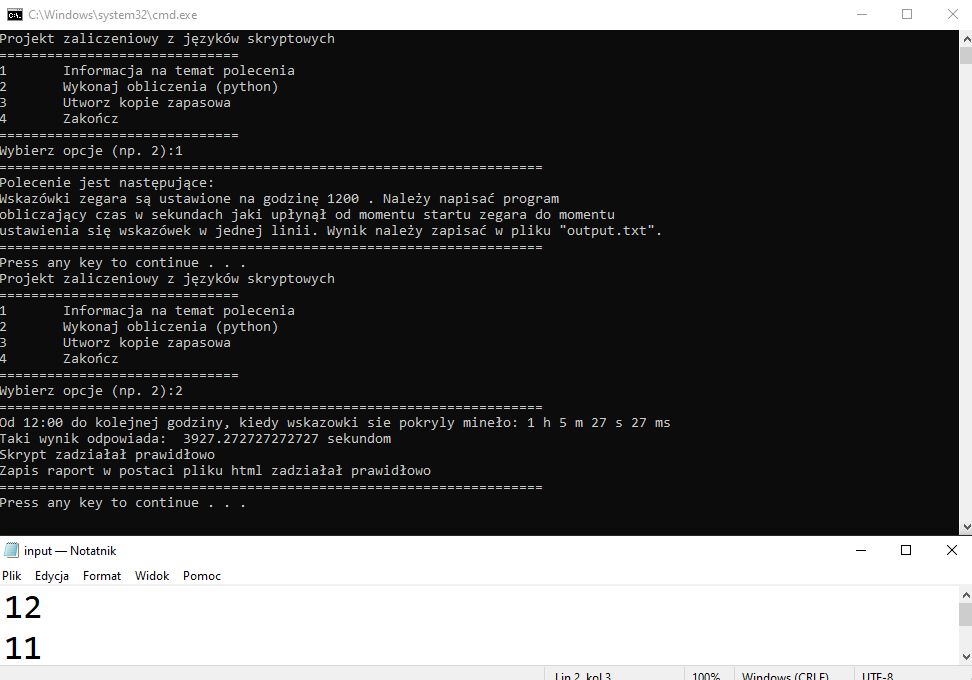
\includegraphics{dzialanie.PNG}
	\end{figure}
	

	
	\newpage
	
    \newpage
	\section{Podsumowanie}
	
	\subsection{Co zostało zrobione}
	\begin{blockquote}
        Program pozwala wczytać wyprowadzone dane, potrzebne do obliczenia czasu, po którym wskazówki zegara ustawią się  jednej linii. Problem matematyczny nie był, aż tak trudny w tym zadaniu co pozwoliło skupić się na integracji skryptów i utrwalenia wiedzy zdobytej w trakcie nauki języków skryptówych.
    \end{blockquote}
    \subsection{Pomysły dotyczące rozbudowy}
	\begin{blockquote}
        Ciekawym pomysłem jest stworzenie animacji w pythonie, zależną od danej godziny, minuty i sekundy która pokazywałaby jak wskazówki poruszają się po tarczy zegara.
    \end{blockquote}

    		\begin{figure}[!htb]
	    \centering
	    output.html
	    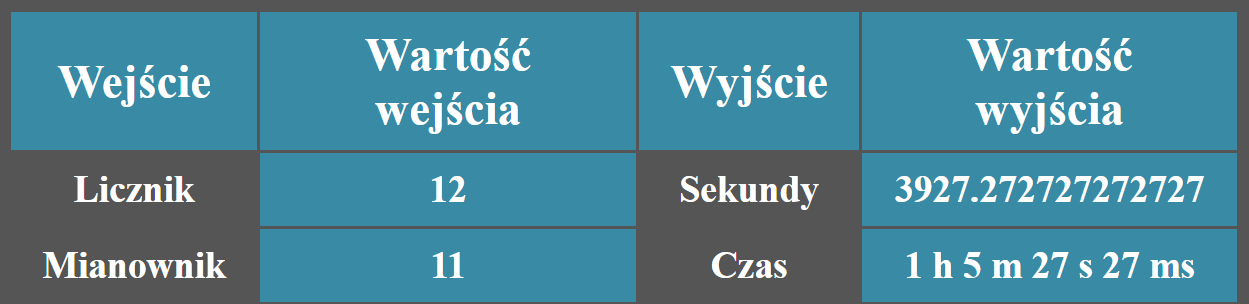
\includegraphics[scale=0.25]{htmlout.PNG}
	\end{figure}


\end{document}
